\documentclass{article}
\usepackage{multirow}
\usepackage{Sweave}
\begin{document}
\Sconcordance{concordance:draft1.tex:draft1.Rnw:%
1 2 1 1 0 4 1 1 8 59 1 1 11 13 1 1 8 17 1 1 8 299 1}




\section*{Abstract}

Community-driven online question and answer forums (CQA) contain an expansive amount of crowd-sourced knowledge. Thousands of questions and answers are posted everyday. One such example of a CQA is iFixit's \textit{Answers} forum. This forum features user-asked questions related specifically to device repair, which are answered by both repair experts and everyday users. A reliable measure of the health of these CQAs is question response time. Fast response times enhance user engagement and satisfaction, and increase web traffic. This paper presents a survival analysis of response time, or the time until a question receives its first answer. A Cox proportional hazards model was developed to predict the survival probability of a question, or the probability that a question receives an answer before a certain time. Though several predictors were signficant, the model's predictive accuracy was low ($R^2 = 0.15$). Significant predictors were the device category of the question (questions pertaining to Apple products received answers faster than others (HR = 2.56, 95\% CI = (2.31, 2.82))) and factors related to the question's title (e.g., whether or not it was phrased as a question (HR = 1.31, 95\% CI = (1.22, 1.41))). Future studies can investigate if factors identified as signifcant in this analysis can be generalized to other CQAs. 

%===================================================================================================
%===================================================================================================

\section*{Introduction}

Community-driven online question and answer forums (CQA) are becoming widely-used sources of information. These online platforms feature thousands of user-posted questions and answers, and can receive millions of visits every month. The CQA analyzed in this paper is iFixit's \textit{Answers} forum. Founded in 2003, iFixit's mission is to equip users with the knowledge and tools to repair their broken devices, as part of an effort to save money and reduce electronic waste. This company provides over 30,000 free online repair guides and sells the specialized tools and parts needed for such repairs.
    
As not all possible repairs are covered in the published guides and users may have additional questions related to existing guides, iFixit's \textit{Answers} forum is another important resource. This platform features questions pertaining to over 9,000 devices, ranging from jammed zippers to shattered iPhone screens and faulty vehicle air conditioners, with over 100,000 solutions. As thousands of users rely on this forum for information, it is important that users receive timely answers. Fast response times enhance user experience and increase web traffic, which is valuable to the reputation and longevity of the \textit{Answers} forum. Analysis of response times can reveal factors that affect how quickly questions receive answers, which can lead to suggestions for how users can ask better questions to minimize response times, and for how the forum design can be improved. 

However, analysis and prediction of response times on CQAs have not been thoroughly investigated. There is need for further analysis of response times in these forums, as the majority of existing research focuses on assessing and predicting question and answer quality. This paper presents a survival analysis on the time until a question receives its first answer on iFixit's \textit{Answers} forum, in order to determine factors significantly related to answer time and to predict the ``survival'' probability of a question.

%===================================================================================================
%===================================================================================================

\section*{Related Work}
  
With the recent increase in the popularity and use of CQAs, these platforms have been the subject of a multitude of studies related to information sciences. Regarding analysis of response times, \cite{Bhat2014} developed a classification model to estimate response times for questions posted on \textit{Stack Overflow}, using both tag-based and textual features. Analysis determine that tag-based features, like the number of ``popular'' tags a question contains or the number of users subscribed to a tag, were the best predictors of response time. \cite{Mahmud} proposed models based on exponential distributions to predict response times, and were built from users' previous wait times for responses. \cite{Rechavi2011} analyzed response times and satisfaction rates for questions posted on \textit{Yahoo Answers!}, and determined that the fastest times were between users who did not follow each other, while the longest times were between users who were mutual friends in the social network. \cite{Asaduzzaman2013} developed a taxonomy for classifying unanswered questions on \textit{Stack Overflow}, and developed a model to predict how long a question would remain unanswered using textual features like title and post length and whether or not the question contained code, and user features, like the number of questions asked and answered by the user prior to posting. The analysis presented in this paper seeks to analyze response time through survival analysis methods, methods that have not yet been investigated or applied to CQAs.  

The majority of existing research has been focused on predicting question and answer quality by using both textual and non-textual features of posts. \cite{Weimer2007} developed a classification algorithm to assess the quality of posts on \textit{Nabble.com}, using primarily textual features (surface, lexical, syntactic, forum-specific, and similarity (relatedness of a post to the topic of the forum) features). \cite{Blumenstock} also determined that textual features, i.e word count, was the most accurate metric of Wikipedia article quality. Wikipedia articles can represent the same kind of user-generated content featured on CQAs. On the other hand, \cite{H.fu} found that non-textual features, like revision and comment count on an answer or the number of points or merit badges a user has, were the most useful indicators of answer quality across four different knowledge domains on \textit{Stack Exchange}. A number of other studies have also developed classification algorithms using both textual and non-textual features with the similar goal of predicting question and answer quality \cite{Yao2015} \cite{Toba2014} \cite{Ponzanelli2014a}. \cite{Ravi2014} presented a slightly different approach by analyzing the content of posts and utilizing latent topic models to predict quality. \cite{Anderson2012} developed models to the long term value of a question and its answers on \textit{Stack Overflow}. The present analysis combines both textual and non-textual features of questions on iFixit's \textit{Answers} forum in a Cox regression model to predict survival probability of questions.

%===================================================================================================
%===================================================================================================

\section*{Materials}

% Table of categorical predictors
\begin{table}[!htbp]
\centering
\begin{tabular}{|p{10cm}|}
  \hline
  Day of the week the question was posted \\ \hline
  Device category the question pertains to. Categories include: Android\/Other Phone, Apple Products, Camera, Electronics, Game Console, Home, Other, PC, Tablet, Vehicle \\ \hline
  Whether or not the question's text contains any end punctuation marks (. ? !) \\ \hline
  Whether or not the question's text is in all lower case \\ \hline
  Whether or not the question's title contains at least one word that is considered ``frequently used'' among answered questions. See appendix for a complete list of these terms. \\ \hline
  Whether or not the question's title contains at least one word that is considered ``frequently used'' among unanswered question. See appendix for a complete list of these terms. \\ \hline
  Whether or not the question's title ends in a question mark \\ \hline
  Whether or not the user edited or added information to the question's text sometime after posting it \\ \hline
  Whether or not the user made an effort to solve the problem prior to asking the question \\ \hline
\end{tabular}
\caption{Categorical predictors derived}
\label{table:categorical}
\end{table}

% Table of quantitative predictors
\begin{table}[!htbp]
\centering
\begin{tabular}{|p{10cm}|}
  \hline
  Average number of characters in each question's tags\\ \hline
  Average tag ``score'' for all of a question's tags. A tag score is defined as the proportion of times a tag appears in all of the data. Questions without tags were assigned a score of 0. \\ \hline
  Number of characters in the question's text \\ \hline
  Number of characters in the user-defined device name \\ \hline
  Ratio of the number of line breaks to the number of characters in the question's text \\ \hline
\end{tabular}
\caption{Continuous predictors derived}
\label{table:continuous}
\end{table}

The data analyzed contained 8,025 questions posted from April 8, 2017 (10:14 PM) to July 7, 2017 (9:28 PM) (the date the data was downloaded). Variables in the data included: device name and category, title, text, tags, whether or not the user was a member of iFixit's site for less than one day before the question was posted, date and time when the question was posted, and date and time when the first answer was received. Variables derived can be found in Table \ref{table:categorical} and \ref{table:continuous}. See appendix for information on how predictors were created. 

%===================================================================================================
%===================================================================================================

\section*{Methods}

Questions analyzed were restricted to those posted in English. The time until event variable used in survival analysis was defined as the time since posting until a question received its first answer. For questions that did not receive an answer by the download date, time until event values were defined as the time since posting to the time the data was downloaded. Such questions were considered right-censored, meaning that exact answer times for these questions are greater than the times in the data (questions can still receive answers after the download date) \cite{Kleinbaum2011}. 

Survival was defined as the event that a question did not receive an answer beyond a certain time, t. Estimates of survival probability were generated with the Kaplan-Meier method, which adjusts to the presence of right-censored, or unanswered questions \cite{Bland1998}. From these estimates, survival curves were constructed to examine the survival experience of questions. Mean, median and other percentiles of survival times were also generated. 

As the probability distribution for response times is unknown, a nonparametric Cox proportional hazards model was developed to predict the survival probability of questions \cite{Moore2010}. To build the model, five-fold cross-validation was used \cite{Rodriguez2010}. Univariate analysis, performed on one training set, was used to identify variables to include in the final predictive Cox model \cite{Hammermeister1979}. Each predictor was entered into univarite Cox models, and strength of association with response times was assessed. Those with partial likelihood ratio test p-values of less than 0.001 were included in the final model. Continuous predictors were entered into univariate Cox models both with and without square root and log transformations to determine the form of the predictor to include into the final model. Univariate analysis was again performed on each continuous predictor to investigate the use of splines. Each predictor, with the transformation found necessary in the previous analysis, was fit to three separate Cox models with restricted cubic splines of three, four, and five knots. AIC statistics were used to determine whether or not to include splines, as well as the optimum number of knots \cite{Harrell2015}. All predictors found to be signficant, along with the transformations and functional forms found to be necessary, were included in the model for cross-validation. No variable selection was used, as \cite{Harrell2015} determined that reducing the number of predictors in the model decreased predictive accuracy more so than leaving all predictors in. 

In each fold of cross-validation, the full model was built on the training set and used to generate predicted hazard ratios on the corresponding test set. To assess prediction performance, predicted hazard ratios were entered into separate Cox models as the single quantitative predictor with response times as the survival time. The resulting Nagelkerke's R-square statistic, concordance statistic, Somers' Dxy, partial likelihood ratio and p-value, were assessed as indicators of the model's performance \cite{Chen}. Signficant results from this model would indicate high predictive accuracy. The partial likelihood ratio assessed is a ratio of the log partial likelihood function evaluated at the parameter estimates, equivalent to a goodness of fit measure of the model with all predictors, and the log partial likelihood function for the null model with no predictors and only the baseline hazard function, equivalent to a goodness of fit measure for the null model. The p-value for this statistic was calculated from the X2 distribution \cite{find}. Concordance statistics and Somers' Dxy are a measure of the model's discriminative ability. Concordance is defined as the probability that for any two randomly chosen questions, the question with the shorter response time also has the higher predicted hazard ratio. Concordance statistics close to 1 indicate high discriminative ability, while statistics close to 0.5 indicate discordance, or random predictions. Somers' Dxy is the difference between the model's concordance statistic and discordance, 0.5. A Somers' Dxy statistic of 0 indicates random predictions, while a statistic equal to 1 indicates perfect predictions \cite{Harrell2015}. These metrics were computed for each iteration on every training and test set. Averages of metrics across training and test sets were evaluated. The final model was then fit to the full data and the same metrics were computed and compared. 

Correlations between scaled Schoenfeld residuals, differences between observed and expected predictor values for questions that received answers, and a function of time, were examined to assess the proportional hazards assumption that the effect of predictors on hazard does not depend on time \cite{Grambsch1994}. Significant correlations would indicate that a predictor has violated this assumption.

To obtain predicted survival probabilities using the model, the predictSurvProb function was used from the pec package. This function uses the Cox model and a vector of times to compute predicted survival probabilities. 

%===================================================================================================
%===================================================================================================

\section*{Results and Discussion}


% Distribution of answer times
\begin{figure}[!htbp]
  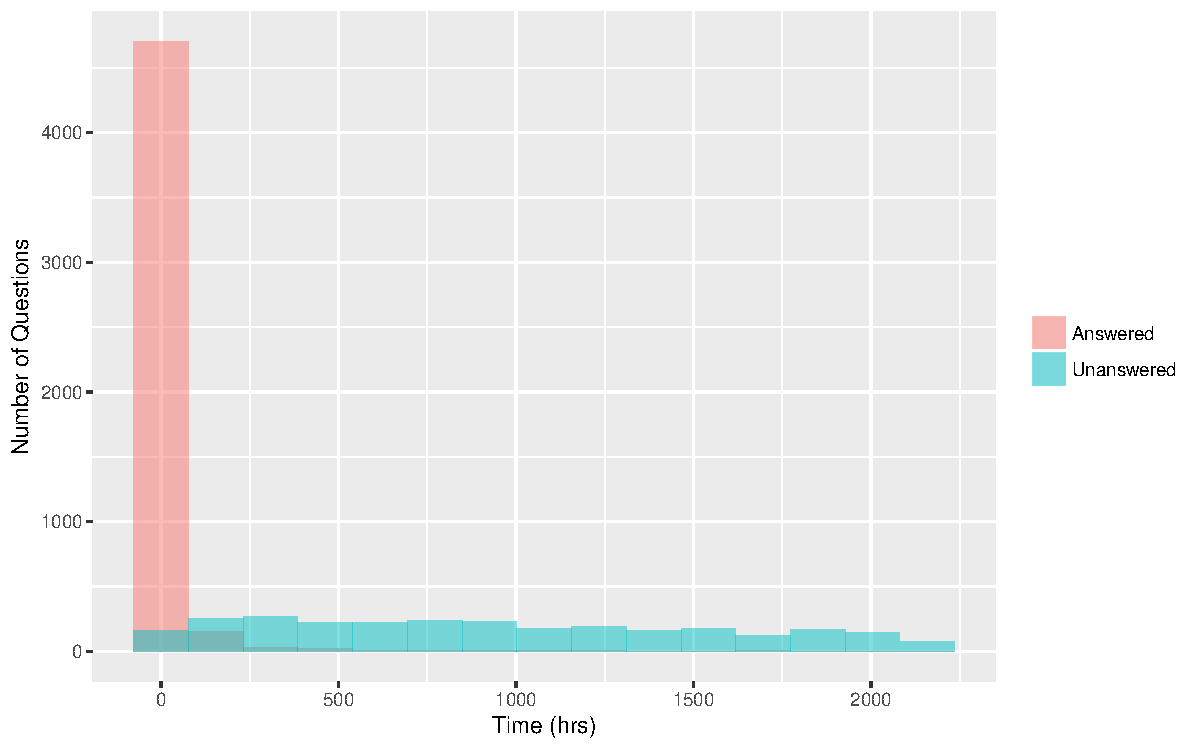
\includegraphics[scale=1]{times_dist.pdf}
  \caption{Distribution of response times}
  \label{fig:answertimes}
\end{figure}

% Kaplan-Meier curve
\begin{figure}[!htbp]
  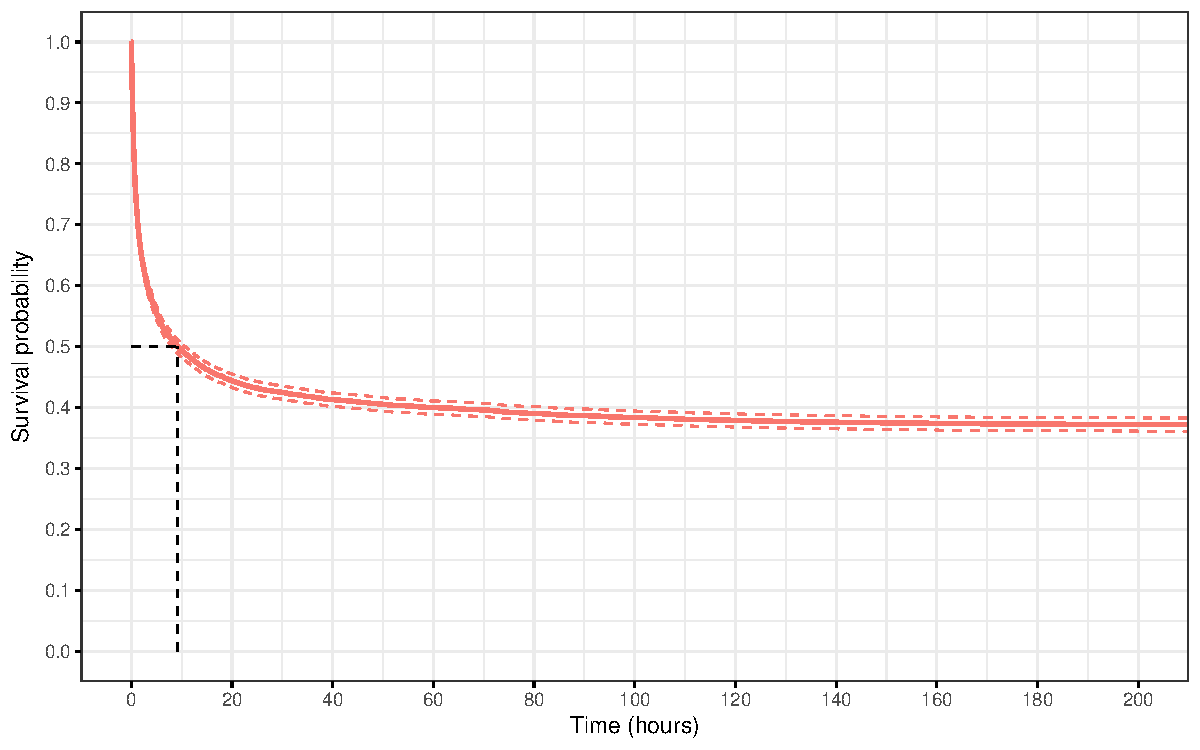
\includegraphics[scale=1]{kmcurve.pdf}
  \caption{Kaplan-Meier curve for all questions}
  \label{fig:kmcurve}
\end{figure}

  Of 8,025 questions in the full data set, 7760 were in English (97\% of the full data). Of those questions, 4951 (63.8}\%) received an answer by the download date. The shortest response time was 0.5 hours. The longest was 2159.02 hours (89.96 days). Figure ~\ref{fig:answertimes} shows the distribution of response times for all questions analyzed. 



% Table of percentiles 
\begin{table}[!h]
\centering
\begin{tabular}{rlr}
  \hline
 Percent\\ Answered & Time (hrs) \\ 
  \hline
  25 & 0.88 \\ 
  50 & 9.16 \\ 
  55 & 18.38 \\ 
  58 & 33.71 \\ 
  60 & 59.47 \\ 
  64 & 683.19 \\ 
   \hline
\end{tabular}
\caption{Kaplan-Meier estimated quantiles of survival time}
\label{table:quantiles}
\end{table}

  Figure  ~\ref{fig:kmcurve} shows the Kaplan-Meier estimated survival probability for all questions in the data. The curve indicates that if a question does not receive an answer within the first 100 hours after it has been posted, the likelihood of it receiving an answer in the future is low. The Kaplan-Meier estimated mean survival time, or the average time until a question received its first answer was 775.75 hours, or 32.32 days. The median survival time, the time at which 50\% of the questions in the data received an answer, was 9.16 hours. Table \ref{table:quantiles} provides additional percentiles of survival time.

% Univariate analysis on quantitative predictors
\begin{table}[!htbp]
\centering
\caption{Univariate analysis results for continuous predictors, ordered by increasing p-values} 
\begin{tabular}{|p{12cm}|p{2cm}|}
  \hline
  Predictor & p-value \\ 
  \hline \hline
  *Log transformation of the number of characters in a question's text & 0.00 \\ \hline
  *Square root transformation of the number of characters in a question's text & 1.1102e-16 \\ \hline
  Number of characters in a question's text (untransformed) & 6.9472e-12 \\\hline
  *Square root transformation of the ratio of the number of line breaks to the number of characters in a question's text & 1.1488e-11 \\ \hline
  *Square root transformation of the average frequency ``score'' of a question's tags & 1.4642e-11 \\ \hline
  Average frequency ``score'' of a question's tags (untransformed) & 1.2706e-08 \\ \hline
  Ratio of the number of line breaks to the number of characters in a question's text (untransformed) & 1.3988e-7 \\ \hline
  *Square root transformation of the number of characters in the user-defined device title & 2.2914e-4 \\ \hline
  *Square root transformation of the average number of characters in a question's tags & 2.9999e-4 \\ \hline
  Number of characters in the user-defined device title (untransformed) & 6.5304e-3 \\ \hline
  Average number of characters in a question's tags (untransformed) & 2.6115e-2 \\ \hline
\end{tabular}
\label{table:qresults}
\end{table}

% Univariate analysis on categorical predictors
\begin{table}[!htbp]
\centering
\caption{Univariate analysis results for categorical predictors, ordered by increasing p-values} 
\begin{tabular}{|p{12cm}|p{2cm}|}
  \hline
 Predictor & p-value \\ 
  \hline \hline
  Day of the week the question was posted & 7.8677e-4 \\ \hline
  Device category & 0.00 \\ \hline
  Whether or not the question's text contained at least one end punctuation mark & 2.5354e-9 \\ \hline
  Whether or not the question's text is in all lower case & 1.5400e-7 \\ \hline
  Whether or not the question's title contains terms considered to be frequently used among answered questions & 7.6397e-5 \\ \hline
  Whether or not the question's title contains terms considered to be frequently used among unanswered questions & 0.00 \\ \hline
  Whether or not the question's title ended in a questionmark & 1.1423e-12 \\ \hline
  Whether or not the user edited or added information to the question's text sometime after posting it & 2.5472e-7 \\ \hline
  Whether or not the user had been a member for less than one day before the question was posted & 0.00 \\ \hline
  Whether or not the user made an effort to solve the problem on their own, prior to asking the question & 3.1648e-5 \\ \hline
  
\end{tabular}
\label{table:cresults}
\end{table}

% Univariate analysis on quantitative predictors
\begin{table}[!htbp]
\centering
\caption{Univariate analysis results for continuous predictors, ordered by increasing p-values} 
\begin{tabular}{| p{5cm} | l | l |}
  \hline
  Predictor & Transformation & p-value \\ 
  \hline
  \multirow{3}{5cm}{Average number of characters in each questions tags}
  & Untransformed & 2.6115e-2 \\ 
  & Log & NA \\
  & Square root & 2.9999e-4 \\ \hline
  \multirow{3}{5cm}{Average frequency score of a question’s tags}
  & Untransformed & 1.2706e-08 \\
  & Log & NA \\
  & Square root & 1.4642e-11 \\ \hline
  \multirow{3}{5cm}{Number of characters in a question's text}
  & Untransformed & 6.9472e-12 \\
  & Log & 0.00 \\
  & Square root & 1.1102e-16 \\ \hline
  \multirow{3}{5cm}{Number of characters in the user-defined device title}
  & Untransformed & 6.5304e-3 \\
  & Log & NA \\
  & Square root & 2.2914e-4 \\ \hline
  \multirow{3}{5cm}{Ratio of the number of line breaks to the number of characters in a question's text} 
  & Untransformed & 1.3988e-7 \\
  & Log & NA \\
  & Square root & 1.1488e-11 \\ \hline
\end{tabular}
\label{table:qresults}
\end{table}


Each training set contained 6208 questions, and each test set contained 1552 questions. Results of univariate analysis, performed on one training set, for transformed and untransformed continuous predictors, and every categorical predictor, are are shown in Table \ref{table:qresults} and Table \ref{table:cresults}, respectively. All categorical predictors and all continuous predictors marked with an asterisk (*) were entered into the full model.

% Splines
\begin{table}[!htbp]
\centering
\caption{Determining the optimal k number of splines for each predictor} 
\begin{tabular}{| p{5cm} | l | l |}
  \hline
  Predictor & K & AIC \\ 
  \hline
  \multirow{ 4 }{ 5cm }{Log transformation of the number of characters in a question's text} 
  & 0 & 65862.83 \\ 
  & 5* & 65862.02 \\ 
  & 4 & 65863.35 \\ 
  & 3 & 65862.08 \\ 
  \hline
  \multirow{ 4 }{ 5 cm }{Square root transformation of the ratio of the number of line breaks to the number of characters in a question's text}
  & 0 & 65890.28 \\ 
  & 5 & 65884.70 \\ 
  & 4 & 65882.98 \\ 
  & 3* & 65881.93 \\ 
  \hline
  \multirow{ 4 }{ 5 cm }{Square root transformation of the average frequency ``score'' of a question's tags}
  & 0* & 65890.75 \\ 
  & 5 & 65891.69 \\ 
  & 4 & 65891.75 \\ 
  & 3 & 65892.35 \\ 
  \hline
  \multirow{ 4 }{ 5 cm }{Square root transformation of the number of characters in the user-defined device title}
  & 0 & 65922.76 \\ 
  & 5* & 65853.56 \\ 
  & 4 & 65882.07 \\ 
  & 3 & 65881.39 \\ 
  \hline
  \multirow{ 4 }{ 5 cm }{Square root transformation of the average number of characters in a question's tags}
  & 0 & 65923.26 \\ 
  & 5 & 65912.11 \\ 
  & 4* & 65910.10 \\ 
  & 3 & 65912.38 \\ 
   \hline
\end{tabular}
\label{table:splines}
\end{table}

Table \ref{table:splines} shows the results of determining the optimal number of knots for each continuous predictor. Values of knots marked with an asterisk (*) were included in the final model. 

% Cross-validation metrics
\begin{table}[!htbp]
\centering
\caption{Average performance metrics for training and test sets} 
\begin{tabular}{rrrrrrrr}
  \hline
 & HR & LR & pval & R2 & Dxy & Concordance \\ 
  \hline
  Training Sets & 2.0164 & 937.2018 & 0.0000 & 0.1401 & 0.2693 & 0.6346 \\ 
  Test Sets & 1.9761 & 220.0417 & 0.0000 & 0.1401 & 0.2584 & 0.6292 \\
   \hline
\end{tabular}
\label{table:cv}
\end{table}

% Final metrics for full data 
\begin{table}[!htbp]
\centering
\caption{Performance metrics for model fit to the full data} 
\begin{tabular}{rrrrrrrr}
  \hline
  HR & LR & pval & R2 & Dxy & Concordance \\ 
  \hline
  2.0010 & 1192.3234 & 0.0000 & 0.1424 & 0.2698 & 0.6349 \\ 
   \hline
\end{tabular}
\label{table:finalmetrics}
\end{table}

Average performance metrics for test and training sets and in Table \ref{table:cv}. Partial likelihood ratio statistics and p-values indicate that the model as a whole is signficantly associated with response time. However, its R^2 statistic and discrimination indexes are considerably low. Metrics did not change significantly from training to test sets, indicating that the model was not overfit. 

% Final model on full data
\begin{table}[!htbp]
\centering
\caption{Coefficients for predictors in the final model} 
\begin{tabular}{|p{1.5cm}|p{6cm}|p{2.5cm}|p{2.5cm}|}
  \hline
 Variable &  Levels & Hazard Ratios & p-value \\ 
  \hline
  \multirow{ 9 }{ 2 cm }{ Device Category } & Apple Product & 0.93 & \multirow{ 9 }{ 1.5cm }{ <0.0001 }\\ 
  & Camera & -0.26 & \\ 
  & Electronics & -0.08 &\\ 
  & Game Console & 0.21 &\\ 
  & Home & 0.39 &\\ 
  & Other & -0.11 &\\ 
  & PC & 0.43 &\\ 
  & Tablet & -0.15 &\\ 
  & Vehicle & 0.38 &\\
  \hline
  & Whether or not the user had been a member for less than one day before the question was posted & -0.10 & 0.0048 \\
  \hline
  & Whether or not the question's title contains terms considered to be frequently used among unanswered questions & -0.27 & <0.0001 \\ 
  \hline
  & Whether or not the question's title contains terms considered to be frequently used among answered questions & 0.05 & 0.2235\\ 
  \hline
  & Whether or not the question's title ended in a questionmark & 0.25 & <0.0001\\ 
  \hline
  & Whether or not the question's text contained at least one end punctuation mark & 0.03 & 0.5348\\ 
  \hline
  & Whether or not the question's text is in all lower case & -0.18 & 0.0052 \\ 
  \hline
  & Whether or not the user edited or added information to the question's text sometime after posting it & 0.28 & 0.0009 \\ 
  \hline
  & Whether or not the user made an effort to solve the problem on their own, prior to asking the question & -0.09 & 0.0137 \\ 
  \hline
  \multirow{ 6 }{ 2 cm }{ Day of the Week } & Monday & 0.01 & \multirow{ 6 }{ 1.5cm }{ 0.0004 }\\ 
  & Saturday & -0.07 & \\ 
  & Sunday & -0.11 & \\ 
  & Thursday & 0.03 & \\ 
  & Tuesday & 0.09 & \\ 
  & Wednesday & 0.10 & \\ 
  \hline
  & Square root transformation of the average frequency ``score'' of a question's tags & 2.23 & 0.0020 \\ 
  \hline
  \multirow{ 3 }{ 2cm }{ Square root transformation of the average number of characters in a question's tags } & _ & -0.08 & 0.0457\\ 
  & avg\_tag\_length' & 0.58 & Nonlinear \\ 
  & avg\_tag\_length'' & -1.52 & 0.0804\\ 
  \hline
  \multirow{ 4 }{ 2cm }{Log transformation of the number of characters in a question's text} & text length & -0.08 & 0.4344
  & text\_length' & -0.36 & Nonlinear \\ 
  & text\_length'' & 2.39 & 0.4578 \\
  & text\_length''' & -3.69 & \\ 
  \hline
  \multirow{ 4 }{ 2cm }{ Square root transformation of the number of characters in a question's device title} & device length & -0.07 & 0.2790 \\
  & device\_length' & 0.18 & Nonlinear \\ 
  & device\_length'' & -0.27 & 0.4185\\ 
  & device\_length''' & 0.21 & \\ 
  \hline
  \multirow{ 2 }{ 2cm }{ Square root transformation of the ratio of number of line breaks to number of characters in a question's text} & line break & 0.12 & 0.3569 \\
  & newline\_ratio' & 0.36 & Nonlinear: 0.6191 \\ 
   \hline
\end{tabular} 
\label{table:coefficients}
\end{table}

Assessing the proportional hazards assumption indicated that several predictors were in violation, results can be found in Table \ref{table:ph_assumption}. Final model statistics and parameter coefficients are in Table \ref{table:coefficients}. Metrics for the final model's performance on the full data are found in \ref{table:finalmetrics}, and are consistent with the metrics found in cross validation---the model as a whole is significantly associated with response time, but has a low $R^2$ statistic and indicates low discriminative ability. Individual predictors found to be significant (alpha = 0.001) are: device category, whether or not the question's text contains ``frequently-used'' terms among unanswered questions, whether or not the questions title ends in a questionmark, whether or not the user updated the question after posting it. 

The data analyzed for this model presented limitations, and may explain the model's low predictive accuracy. Many users on the CQA incorrectly specified the device name in their question (e.g. ``Turtle Beach Ear Force Xmy grandson chewed through the wire while he was playing it's brand-new is there anyway I can have it fixed0 One''), or did not include a device name at all. Many users also incorrectly used the tagging system by including ambiguous and lengthy tags like ``someone sat on it :('' or ``help me please!!!!!''(tags are generally a couple key words that describe the topic of the question). These inconsistencies in the data presented some difficulties in analysis, and may explain the model's low R^2 and discrimination indexes. 

Future studies can further investigate if the predictors found to be significant in this study can be generalized to other CQAs. 

%===================================================================================================
%===================================================================================================


\section*{Conclusion}

This study developed a Cox proportional hazards model to predict the probability that a question posted on iFixit's \textit{Answers} forum receives an answer before a certain time. Predictors found to be signficant in the model included: device category, whether or not the question contained words considered to be ``frequently-used'' among unanswered questions, whether or not the title ends in a questionmark, and whether or not the user updated the question's text after the initial posting. While overall the model was signficant, its predictive performance was considerably low. 


%===================================================================================================
%===================================================================================================


\section*{Acknowledgement}

This research is supported by the Bill and Linda Frost fund. 


%===================================================================================================
%===================================================================================================

\section*{Appendix} 


% Table to display an answered question---------------------------------
\begin{table}[!htbp]
\centering
\begin{tabular}{|p{2cm}|p{3cm}|p{6cm}|{2cm}|{2cm}|{2cm}|{2cm}}
  \hline
 Device & Title & Text & User & Date Posted & First Answer Date & Time until first answer \\
  \hline
  iPhone 6 & iPhone water damage, touch screen issue & So I dropped my iPhone in water 4 days ago. Have done the whole rice thing and seen huge difference in it. However, only one side of my screen works and it is the one side which I need to unlock the phone. What would be the best way forward? & 1 & 2017-05-10 21:50:48 GMT & 2017-05-10 23:12:27 & 1.361 hr \\ 
   \hline
\end{tabular}
\caption{Example of an answered question}
\label{table:answered_q}
\end{table}

% Table to display an unanswered question-------------------------------
\begin{table}[!htbp]
\centering
\begin{tabular}{|p{2cm}|p{3cm}|p{6cm}|{2cm}|{2cm}|{2cm}|{2cm}}
  \hline
 Device & Title & Text & User & Date Posted & First Answer Date & Time until first answer \\
  \hline
  android tablet & ccccaaaan you help me fix my touch screen & touch screen not worki & 0 & 2017-05-23 07:35:12 GMT & NA & NA \\ 
   \hline
\end{tabular}
\caption{Example of an unanswered question}
\label{table:unanswered_q}
\end{table}
%-----------------------------------------------------------------------


Device category 

\begin{itemize}
  \item Original device categories, defined by iFixit, included: Apparel, Appliance, Camera, Car and Truck, Computer Hardware, Electronics, Game Console, Household, Mac, Media Player, PC, Phone, Skills, Tablet, Vehicle. Device titles were parsed and certain categories were combined or separated to create a new device categorization. Categories in the final variable included: Android/Other Phone, Apple Product, Camera, Electronics, Game Console, Home, Other, PC, Tablet, Vehicle. Under original device categorization, 1,954 questions (25.2\% of 7,760) were not categorized correctly and indicated an NA for its category. Missing values were a result of users creating questions for devices not already in the iFixit's database, or from the user incorrectly defining the device name. For questions with missing categories, key words were searched for in device titles to recategorize accordingly. 
\end{itemize}

%-----------------------------------------------------------------------

Whether or not the question's title contains terms considered to be frequently used among answered/unanswered questions

\begin{itemize}
  \item Logical variables indicating true if a question's title contained at least one of the words in the ``frequently-used'' words list for answered and unanswered questions, respectively. 
  \item These variables were created based on the hypothesis that certain question topics are more popular among the answering community, and that questions concerning these topics might receive an answer faster than questions that do not. Similarly, certain topics might be unpopular, and questions pertaining to those topics might receive answers slower than those that do not (cite).
  \item To create the variables, the data was separated between answered and unanswered questions. For the data frame containing answered questions, text mining techniques were used to create a list of every word within each questions' titles and the frequency, or proportion of times those words occurred among all answered questions' titles. The same was performed for the data frame containing unanswered questions. ``Frequently-used'' words in answered questions were defined as those that appeared in more than 1\% of all answered questions' titles, and appeared in more answered questions than in unanswered questions. To determine the latter, a ratio of frequencies, or proportions of times a word occurs, was assessed. The ratio was calculated as the proportion of time a word occured among answered questions, to the proportion of times a word occured in unanswered questions. As an example, if ``cracked'' appeared in 2\% of answered questions and 0.1\% of unanswered questions, it would be considered ``frequently-used'' among answered questions as it occurs in more than 1\% of answered questions' titles and occurs 20 times more in answered question than in unanswered questions (ratio = 0.02/0.001 = 20). Similarly, ``frequently-used'' words in unanswered questions must occur in 1\% or more of all unanswered question's titles and occur in more unanswered questions than answered questions. As there was some overlap between ``frequently-used'' words in each list and the device categories, every word that matched a device name was removed from the lists. The resulting list for answered questions contained 111 words. The list for unanswered questions contained 32 words. Lists can be found in Table \ref{table:frequent_terms}
\end{itemize}

%--------Table with list of frequently used words------------------------
\begin{table}[!htbp]
\centering
\caption{Lists of ``frequently-used'' terms among answered and unanswered questions' titles, ordered by decreasing frequency}
\begin{tabular}{|p{4cm}|p{8cm}|}
  \hline
 ``Frequently-used'' terms among answered questions & screen, turn, working, replacement, power, work, replace, charging, charge, button, touch, black, turning, broken, start, stuck, new, lcd, upgrade, problem, change, port, replaced, card, open, boot, replacing, remove, reset, back, drive, error, cable, ssd, cracked, hard, one, dropped, logic, lines, white, keeps, pro, dead, now, front, damage, switch, parts, glass, still, charger, issue, sim, turns, digitizer, just, mode, model, backlight, usb, stopped, logo, starting, know, unresponsive, password, factory, call, use, damaged, find, sensor, possible, fixed, side, galaxy, data, ipod, problems, issue, slow, system, connector, without, overheating, code, ram, air, microphone, please, red, much, plugged, getting, booting, left, way, buy, plus, time, loose, lock, coming, got, shuts, says, install, key, door, top \\
  \hline
  ``Frequently-used'' terms among unanswered questions & sound, light, wifi, speaker, connect, picture, stay, noise, bluetooth, isnt, apps, going, rear, question, play, stop, service, take, hear, lights, showing, network, volume, come, keep, connection, flashing, shut, print, blue, buttons, edit \\ 
   \hline
\end{tabular}
\label{table:frequent_terms}
\end{table}

%-----------------------------------------------------------------------

Whether or not the question's title ended in a questionmark

\begin{itemize}
  \item This variable was created based on the hypothesis that questions with titles in the form of questions receive answers faster than those that do not.
\end{itemize}

%-----------------------------------------------------------------------

Whether or not the question's text contained at least one end punctuation mark

\begin{itemize}
  \item This variable was created to investigate if run-on sentences, sentences with no end punctuation, take longer to receive an answer. 
\end{itemize}

%-----------------------------------------------------------------------

Whether or not the user made an effort to solve the problem on their own, prior to asking the question

\begin{itemize}
  \item Logical variable indicating true if the asker included words in the question's text that indicate prior effort or research was done before asking the question (e.g. ``tried'', ``attempted'', ``tested''). This variable was created based off of findings from \cite{Bhat2014}. 
\end{itemize}

%-----------------------------------------------------------------------

Average frequency ``score'' of a question's tags

\begin{itemize}
  \item This variable was created to investigate the idea that some tags are more ``popular'', or widely used than other tags, and that including such tags might increase the likelihood of that question receiving an answer faster. This variable is the average frequency, or proportion of times a question's tags appear in all of the data set. If a question has a higher average, than at least one of it's tags are frequently used. This variable was created based off of findings from \cite{Bhat2014}. 
\end{itemize}

%-----------------------------------------------------------------------

Number of characters in the user-defined device title

\begin{itemize}
  \item This variable was included to capture when a user incorrectly defines the device name. For example, the device variable for question 390271 is, “Turtle Beach Ear Force Xmy grandson chewed through the wire while we was playing it's brand-new is there anyway I can have it fixedO One”, and is 136 characters long. 11 questions in the data also did not include any device title. This variable was created based on the intuition that users who incorrectly define their devices, or do not include any device title, make it difficult for the answering community to discern the question's topic, and thus have longer answer times or remain unanswered.
\end{itemize}

%-----------------------------------------------------------------------

Average number of characters in a question's tags

\begin{itemize}
  \item This variable, similar to the device-length variable, was created to capture when a user correctly or incorrectly used the tagging system. For example, question 390989 included the tag tag: “i need to repair the headset because i can not find the bluetoot”, which is 64 characters. Question 410254 includes tags "sound", "sound driver" and "speaker" and has an average of 8 characters per tag. It is hypothesized that users who correctly define tags, as with the latter user, receive answers quicker than the former. 
\end{itemize}

%-----------------------------------------------------------------------

Ratio of the number of line breaks to the number of characters in a question's text

\begin{itemize}
  \item This variable was based on the hypothesis that question's that include line breaks in the text are generally easier to read than questions that don't include any, and thus have faster answer times. 
\end{itemize}



\bibliography{questions}
\bibliographystyle{ECA_jasa}









\end{document}
